\newpage
\section{509. 斐波那契数}
\label{leetcode:509}

\subsection{题目}

\textbf{斐波那契数},通常用 F(n) 表示,形成的序列称为\textbf{斐波那契数列}。
该数列由 0 和 1 开始,后面的每一项数字都是前面两项数字的和。也就是:

\begin{verbatim}
  F(0) = 0,   F(1) = 1
  F(N) = F(N - 1) + F(N - 2), 其中 N > 1.
\end{verbatim}

给定 N,计算 F(N)。

\textbf{示例 1}:

\begin{verbatim}
  输入:2
  输出:1
  解释:F(2) = F(1) + F(0) = 1 + 0 = 1.
\end{verbatim}

\textbf{示例 2}:

\begin{verbatim}
  输入:3
  输出:2
  解释:F(3) = F(2) + F(1) = 1 + 1 = 2.
\end{verbatim}

\textbf{示例 3}:

\begin{verbatim}
  输入:4
  输出:3
  解释:F(4) = F(3) + F(2) = 2 + 1 = 3.
\end{verbatim}

\textbf{提示}:

  $0 \leq N \leq 30$

\subsection{题目解析}

这个题目非常重要,后面的爬楼梯,硬币兑换都是这个题目的变种。

DP 方程如下:

  dp[0] = 0 \\
  dp[1] = 1 \\
  dp[i] = dp[i-1] + dp[i-2], $i \geq 2$

\subsection{参考题解,傻递归}

这种方法的状态树巨大,时间复杂度是 O(2$^{n}$)。

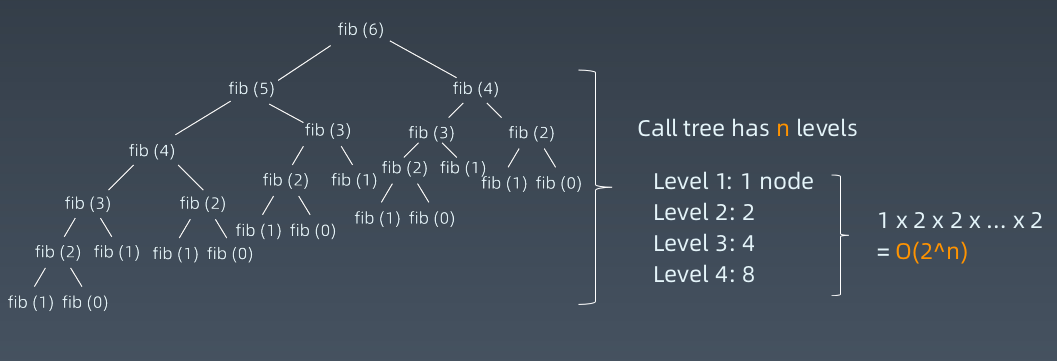
\includegraphics[width=140mm,height=60mm]{images/leetcode/leetcode_509_01.png}

\begin{verbatim}
/**
 * @param {number} N
 * @return {number}
 */
var fib = function(N) {
  if (N < 2) { return N; }
  return fib(N-1) + fib(N-2);
};
\end{verbatim}

\subsection{参考题解,递归+缓存}

时间复杂度为 O(n)。\\
空间复杂度 O(n)。

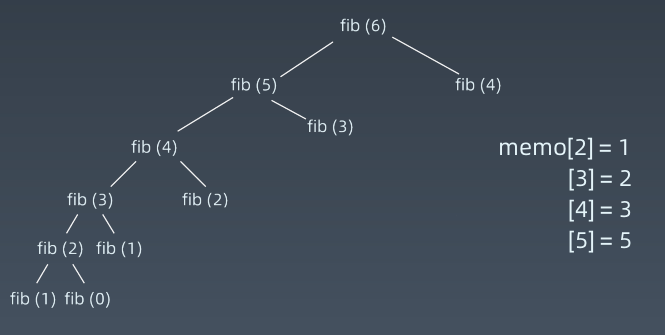
\includegraphics[width=100mm,height=50mm]{images/leetcode/leetcode_509_02.png}

\begin{verbatim}
/**
* @param {number} N
* @return {number}
*/
var fib = function(N) {
  const m = new Map();
  m.set(0, 0);
  m.set(1, 1);
  return recursion(N, m);
};

function recursion(N, m) {
  if (m.has(N)) {
    return m.get(N);
  }
  const result = recursion(N-1, m) + recursion(N-2, m);
  m.set(N, result);
  return result;
}
\end{verbatim}

\subsection{参考题解,递推1}

开辟一个状态数组。

时间复杂度 O(n)。\\
空间复杂度 O(n)。

\begin{verbatim}
/**
* @param {number} N
* @return {number}
*/
var fib = function(N) {
  if (N < 2) { return N; }
  let dp = new Array(N+1);
  dp[0] = 0;
  dp[1] = 1;
  for (let i = 2; i <= N; i += 1) {
    dp[i] = dp[i-1] + dp[i-2];
  }
  return dp[N];
};
\end{verbatim}

\subsection{参考题解,递推经典解法}

上一种解法,你可以看到在 for 循环里面,每次的操作
其实就只涉及到 3 个变量的操作,所以我们其实是可以
不用开辟这个数组的。我们只需要每次循环都保存一下
最新的状态即可。

时间复杂度 O(n)。\\
空间复杂度 O(1)。

\begin{verbatim}
/**
 * @param {number} N
 * @return {number}
 */
var fib = function(N) {
  if (N < 2) {
    return N;
  }
  let f1 = 0;
  let f2 = 1;
  for (let i = 2; i <= N; i += 1) {
    [f1, f2] = [f2, f1 + f2];
  }
  return f2;
};
\end{verbatim}

\subsection{参考题解,查表法}

因为题目中说了 N 的范围是 0 到 30,所以这个
范围比较小,我们可以事先把答案算出来,然后查表。

时间复杂度 O(1)。\\
空间复杂度 O(n)。

\begin{verbatim}
/**
 * @param {number} N
 * @return {number}
 */
var fib = function(N) {
  return fibArray[N];
};

const fibArray = [
       0,      1,      1,      2,      3,
       5,      8,     13,     21,     34,
      55,     89,    144,    233,    377,
     610,    987,   1597,   2584,   4181,
    6765,  10946,  17711,  28657,  46368,
   75025, 121393, 196418, 317811, 514229,
  832040
];
\end{verbatim}

\subsection{参考题解,矩阵法}

时间复杂度 O(${\log}_2 n$)。\\
空间复杂度 O(1)。

\subsection{参考题解,通项公式}

时间复杂度 O(1)。\\
空间复杂度 O(1)。

通项公式:

\begin{displaymath}
  f(n) = \frac
  {{ \frac{1 + \sqrt{5}}{2} }^{n} - { \frac{1 - \sqrt{5}}{2} }^{n}}
  {\sqrt{5}}
\end{displaymath}

\begin{verbatim}
/**
* @param {number} N
* @return {number}
*/
var fib = function(N) {
  return Math.round((Math.pow((1 + Math.sqrt(5))/2 , N) -
      Math.pow((1 - Math.sqrt(5))/2, N)) / Math.sqrt(5));
};
\end{verbatim}

\subsection{题目扩展1}

T0 = 0, T1 = 1, T2 = 1, 且在 n >= 0 的条件下 Tn+3 = Tn + Tn+1 + Tn+2

详细见题目 \hyperref[leetcode:1137]{1137. 第 N 个泰波那契数}

\subsection{题目扩展2}

如果相邻的步数不能相同,要怎么办?下面这是个人思考,不一定正确。

\begin{verbatim}
/*
n = 5, steps = 1, 2
0
1 1
2 2
3 1+2, 2+1
4 1+2+1
5 2+1+2
   0  1  2  3  4  5
1  0  1  n  1  1  n
2  0  n  1  1  n  1


n = 5, steps = 1, 2, 3
0
1 1
2 2
3 3, 1+2, 2+1
4 3+1, 1+2+1, 1+3
5 1+3+1, 3+2, 2+1+2, 2+3
   0  1  2  3  4  5
1  0  1  n  1  2  1
2  0  n  1  1  n  2
3  0  n  n  1  1  1
*/
\end{verbatim}

\begin{verbatim}
function superfib(n, steps) {
  let states = new Array(steps.length).fill(null).map(() => {
    return new Array(n+1).fill(null);
  });

  for (let col = 1; col <= n; col += 1) {
    for (let row = 0; row < steps.length; row += 1) {
      let step = steps[row];
      let preCol = col - step;
      if (preCol < 0) {
        continue;
      }
      if (preCol === 0) {
        states[row][col] = 1;
        continue;
      }

      let preSum = 0;
      for (let preRow = 0; preRow < steps.length; preRow += 1) {
        if (preRow !== row && states[preRow][preCol] !== null) {
          preSum += states[preRow][preCol];
        }
      }
      if (preSum > 0) {
        states[row][col] = preSum;
      }
    }
  }

  let result = 0;
  for (let row = 0; row < steps.length; row += 1) {
    if (states[row][n] !== null) {
      result += states[row][n];
    }
  }
  return result;
}

const n = 5;
const steps = [1,2,3];
const result = superfib(n, steps);
console.log(result);
\end{verbatim}
